\section{System Design}
\label{sec:design}
\subsection{Backlight Scaling Algorithms}
The basic idea of luminance compensation is when the backlight is
dimmed, the luminance of frame pixels are enhanced. Thence the power
savings are achieved while no observable distortion exists. In next
sections, we denote the $t = 1, 2, ...$ as the frame index in a live
streaming. And the $Y_{t}^{max} \in [0, 255]$ is the max luminance of
frame $t$. The $b_{t} \in [0, 1]$ stands for the target backlight
level when the $t$th frame is rendering.

\subsubsection{Dynamic Programming}
Although the ideal case is the pixels of the $t$th frame are enhanced by
$(255 - Y_{t}^{max})$, so that the $b_{t}$ can be scaled to
$\frac{Y_{t}^{max}}{255}$, which is the minimum possible value, 
without losing any observable fidelity. However, if we do this
practically, two negative phenomenons are found:
\begin{itemize}
  \item{The {\it flickering} is found as the screen backlight varies
    dramatically.}
  \item{On devices, The backlight scale can't react in real-time
    manner. The hardware response the scaling directive in a short
    delay.}
\end{itemize}
Both of the facts should be taken into account when we scale the
backlight. Since it is so, we quantify the next three
constraints. With the $\Delta_{b}$, which stands for the max allowed
backlight difference in one adjustment operation, we have
$b_{t+1} \in [b_t \times (1 - \Delta_t), b_t \times (1 + \Delta_t)]$.  And another
constraint is the $l_{min}$, which stands for the frame number which
must keep same backlight level. The last one is that $b_{t} <
\frac{Y_{t}^{max}}{255}$, keeping the backlight level in its $[0,1]$
range.  its . we will get the Dynamic Programming solution from this
recurrence:
$$ B(t,b) = \min_{t',b'}(b \times (t - t') + B(t', b')) $$

More explanations later...

\subsubsection{Greedy}
The DP algorithm certainly can offer us the best solution on adjusting
the backlight over the frames. And the greedy version can also help
achieve the similar effect. Except that we have to render some frames
in distortion without violating the constraints.

\begin{algorithm}
  \caption{the greedy algorithm}
  \label{alg:greedy}
  \begin{algorithmic}[1]
    \LineComment{On input $(t, Y_{t}^{max}, b_{old})$, where $b_{old}$
      is the adjusted backlight value of last time, we generate
      $(Y_{t}', b_{t})$, where the $Y_{t}'$ is how many the $t$th
      frame should enhance its pixels. Also the $b_{old}$ is updated
      by $b_t$}
    \\
    \If {$t = 1$}
      \State $b_{old} \gets Y_{t}^{max} / 255$
      \State $Y_{t}' \gets 255 - Y_{t}^{max}$
      \State $b_{t} \gets b_{old}$
      \Return $(Y_{t}', b_t)$
    \EndIf
      \\
      \State $b_{t}' \gets Y_{t}^{max} / 255$
    \If {$b_{t}' < b_{old} - \Delta_{b}$}
      \State $b_{old} \gets b_{old} - \Delta_{b}$
    \ElsIf {$b_{t}' > b_{old} + \Delta{b}$}
      \State $b_{old} \gets b_{old} + \Delta_{b}$
    \Else
      \State $b_{old} \gets b_{t}'$
    \EndIf
    \\
    \State $Y_{t}' \gets 255 - 1 / b_{old}$
    \State $b_{t} \gets b_{old}$\\
    \Return $(Y_{t}', b_{t})$
  \end{algorithmic}
  
\end{algorithm}

In this the algorithm~\ref{alg:greedy}, we input the luminance
$Y_{t}^{max}$ of $t$th frame and get the target backlight level
$b_{t}$ for future adjustment. Then we can scale the backlight when
the corresponding frame is shown on the display. However, the distortion
may occur if the $t$th frame has the max luminance $Y_t^{max}/255 >
b_{old} + \Delta_b$.

%% \begin{itemize}
%%   \item
%%     {
%%       Local DP.
%%     }
%%   \item
%%     {

%%       right-bottom is not significant

%%       set the pixels around the frame. if it doesn't match, select the
%%       most candidate or the last one. 
%%     }
%%   \item
%%     {
%%       skipping some frames.
%%     }
%% \end{itemize}

%% It's not so effective if we process per frame at the receiving end and


\subsection{System Design}
 %% put the components at both sender
%% side and receiver side.
%% The scanning module and the
%% adjusting module, respectively resides in sender and receiver. For the
%% sender, before encoding, we insert the scanning module at this
%% point. it is responsible of scanning generate the raw frames collected
%% from the capturer, usually is the camera on the mobile. Actually two
%% options for the scanning model locations are available. One is the
%% point we mentioned. The second one the at the receiver side. But as we
%% know, the frames have to be composed at the time of rendering. So if
%% we scan the raw frames received, we have to scan $n$ times per frame,
%% which is simply impossible. The alternative option is to scan the
%% composed frame at rendering time. 1) the time is not enough if the
%% scanning operation is more time consuming than the $\frac{1}{fps}$. 2)
%% No space for DP. So the first option is not the only choice, but it's
%% the better one.
The system logically contains three components. The first one is the
{\bf Scanning module}, which is responsible of scanning YUV frames for
liminance information.  Unlike the case of playing VOD or local
Videos, real-time communication is featured both frame generation and
frame rendering. Hence this module can either locate at sender side,
before the encoder, or receiver side, after the decoder. The sender is
an evidently better option. If the Scanning module sits at the
receiver side, thinking of the scenario where $N$ users are involved
in a video conference, each client have to scan $N$x frames. To also
reduce the frame number to $1$ per frame at the receiver side, the
system can only scan the composed frame at rendering time. This makes
the time too stringent and the DP is not a option for adjust backlight
any more. Further, the scaling operation always got behind with
rendering operation due the hardware constraint. After scanning, the
max luminance information is hidden inside corresponding frame. To
avoid packet loss in network transfer, we set the max luminance value
at all four corners. When these values are fetch out, the most
equivalent value is elected as the max luminance of this frame.

\begin{figure}[!htb]
  \centering
  \label{fig:design}
  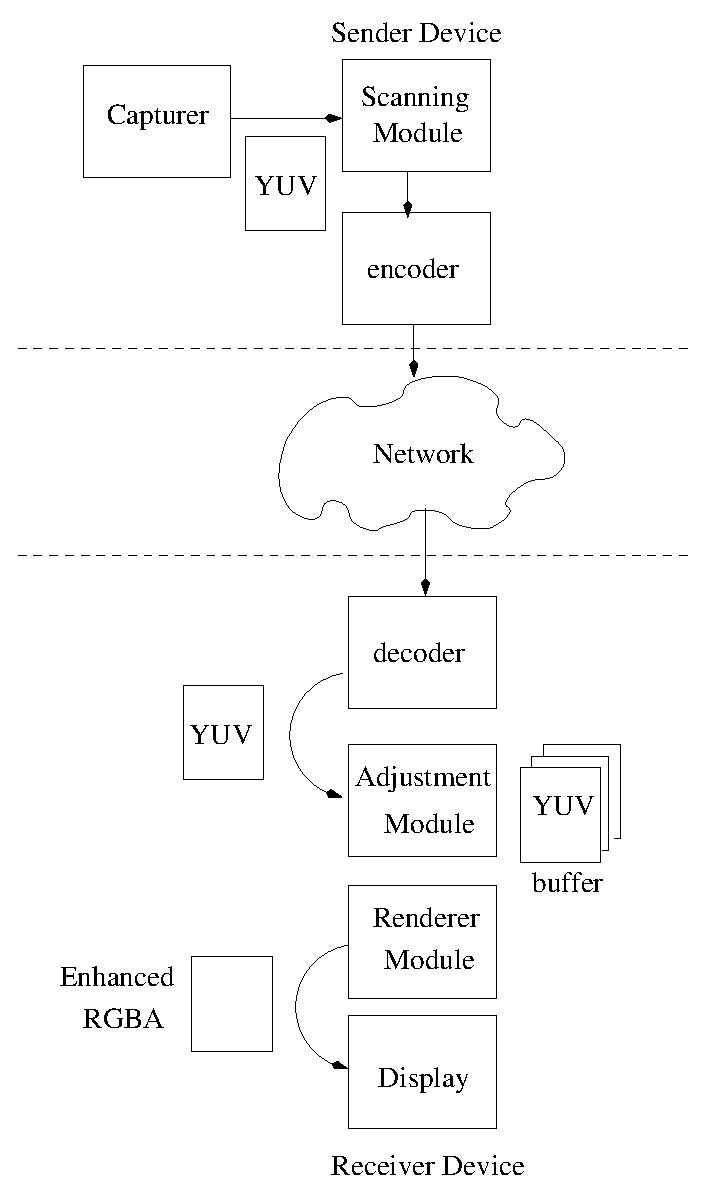
\includegraphics[scale=.5]{./figures/design.eps}
  \caption{System Design}
\end{figure}

We intend to use CPU other than GPU to scan the raw frame. 1)
practically the resolution and fps in real-time communication
streaming is usually lower than other stream case. CPU is completely
capable of doing this in time. 2) The GPGPU and technique has little
threads priority mechanism, especially on the mobile platform. While
another GPU-related task(YUV conversion and frame composition) has
obviously higher priority is most likely to be occupied. 


The second component is the {\bf Adjustment Module}. This component
can buffer the frames, fetch out luminance information and then
perform the adjustment. The resulting values of brightness are sent to
the next module for following rendering. The module locates the
receiver side to avoid built another channel over the network for
passing the adjusted brightness values. The strategy used to adjust
brightness is chosen between the DP and Greedy mentioned before.

%% adjust the space of pixels to emluminance and also notice the system
%% to scale its backlight. What I need mention is that if we have to
%% perform the DP, we have to equip a queue of size greater than
%% $1$. two reason we prefer the Greedy version.
%% 1) The network bandwidth throttle the size of queue. make it hardly
%% achieve global optimization in backlight scale. 
%% 2) In the case of real-time communication, the variation of scenarios
%% is little. We hardly meet the case of luminance raise or drop
%% abruptly.

The third component is the {\bf Rendering Module}. For the system which
already has the function of conversion between YUV and RGBA frames,
plug the function of lightening pixels just before this
conversion. Also this module is responsible of sending the backlight
scaling requests to OS at the appropriate time point so that display
can be correctly compensated. 
%%  of frame $t$ by  of When the frames are composed and
%% before convert to RGBA format in shader. we increase the Y component. 

%% unlike the streaming or local video play case, the real-time
%% communication need compose several frames together(e.g, in
%% peer-to-peer case, typically the opponent's head occupy the most
%% display and the picture of the users lay at the bottom of display).
%% we must efficiently compose these pictures together in using GPU
%% without dropping the fps. Finally, we don't need risk the high power
%% consumption difference between GPU on-and-off. We only afford the
%% extra computation power consumption.

\section{implementation}
\label{sec:implementation}

We built our system base on AppRTC, which is part of the project
chromium. This Android app links to libjingle.so, which is the WebRTC
support library of Chrome browser. The scanning module and adjustment
module resides inside the libjingle.so and Rendering module is part of
the Android app.



